\documentclass{article}

\usepackage{graphicx}
\usepackage{tikz}
\usepackage{tikzsymbols}
\usetikzlibrary{calc,patterns,shapes.geometric}
\pagestyle{empty}
\usepackage[margin=0pt]{geometry}
\geometry{papersize={14in,12in}}

\def\centerarc[#1](#2)(#3:#4:#5){\draw[#1] ($(#2)+({#5*cos(#3)},{#5*sin(#3)})$) arc (#3:#4:#5);}

\begin{document}
	\begin{figure}
		\centering
		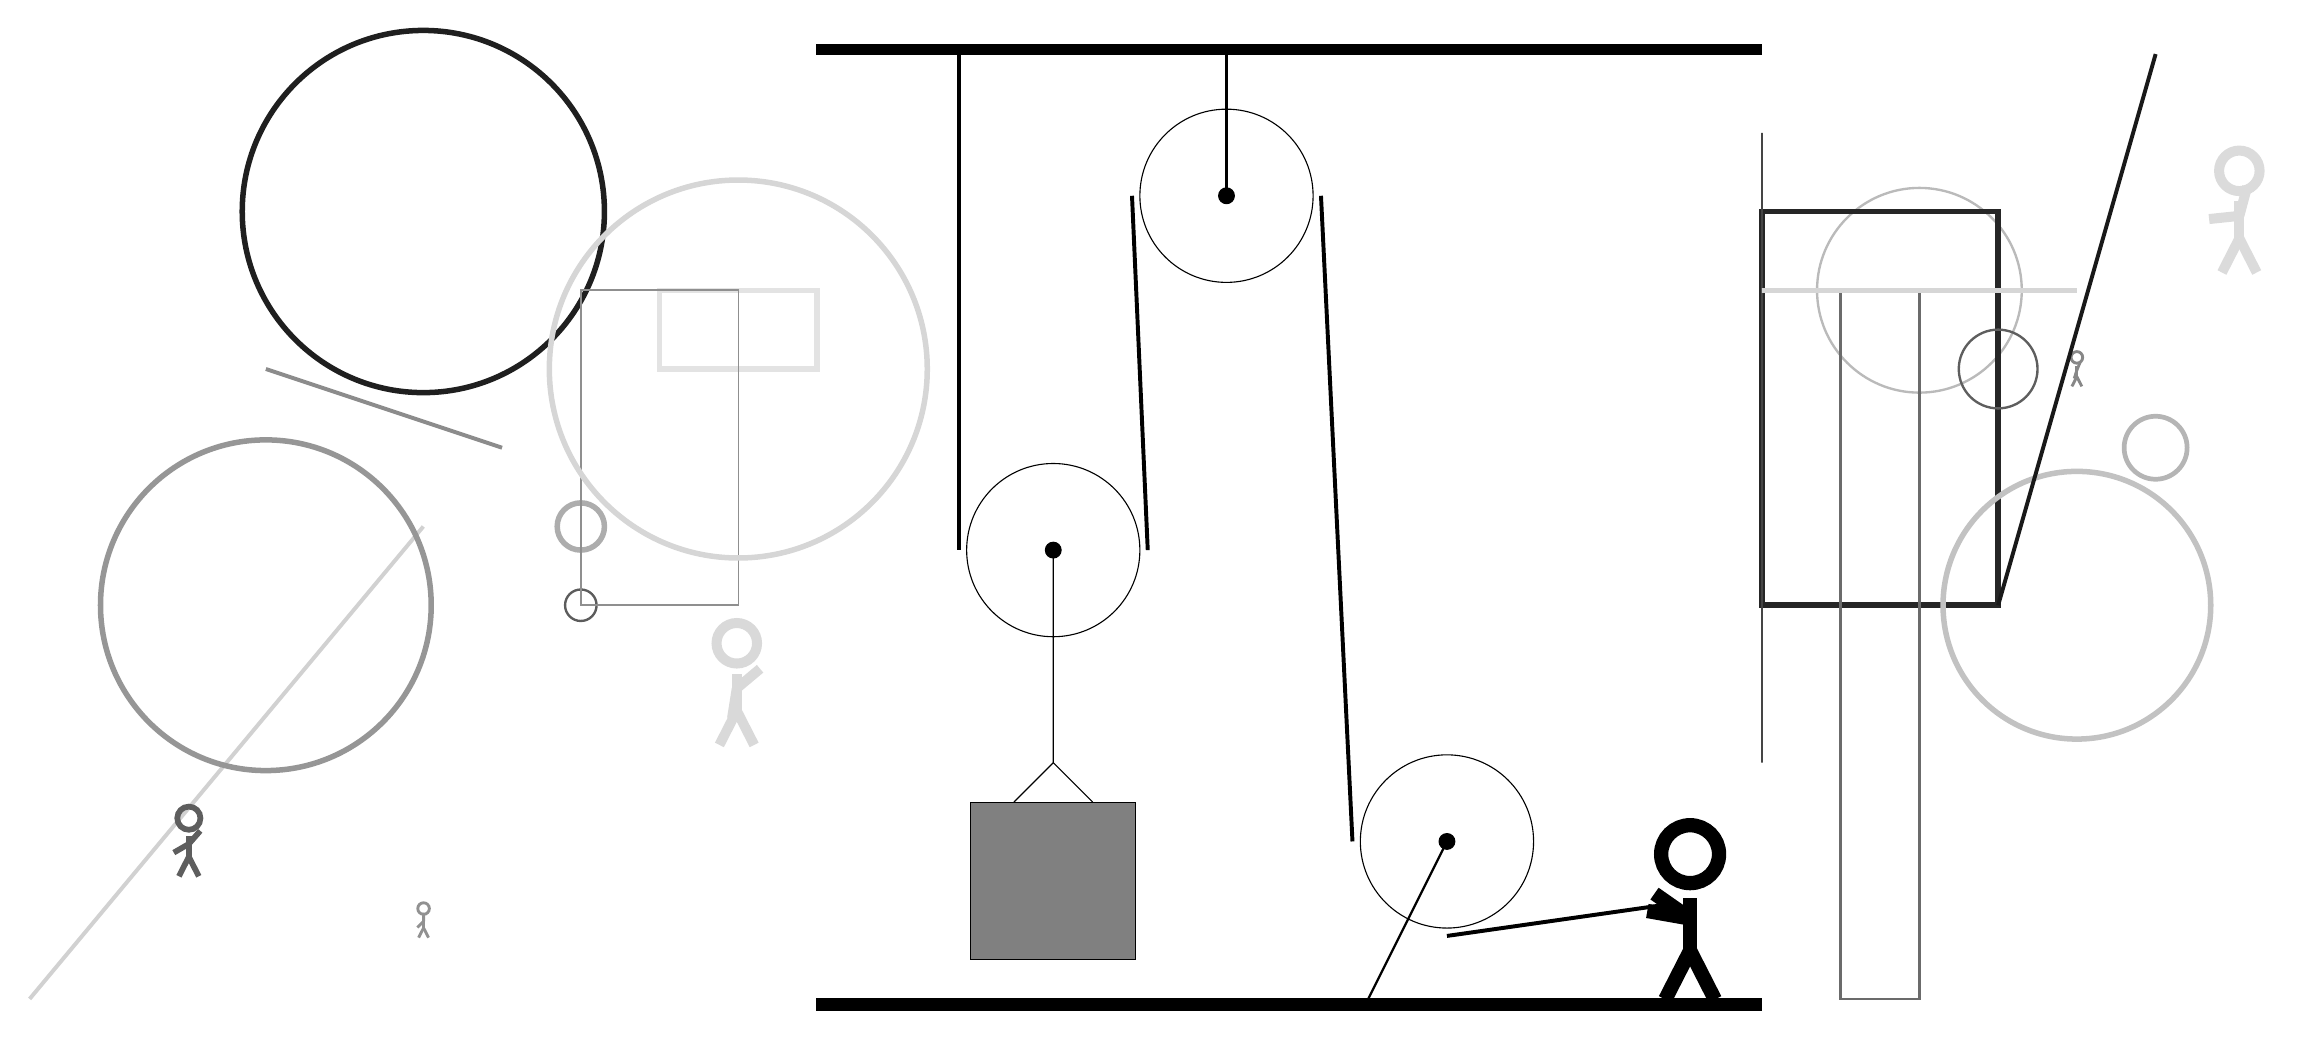
\begin{tikzpicture}
			%%%%% START %%%%%
			
			\draw[fill=black] (-2, 9) rectangle (10, 9.125);
			
			\draw (3.2, 7.2) circle (1.1);
			\draw[fill=black] (3.2, 7.2) circle (0.1);
			\draw[thick] (3.2, 7.2) -- (3.2, 9);
			
			\draw [line width=0.3mm, color=black!27](12, 6) circle (1.3);
			
			\draw[line width=0.7mm, color=black!85] (10, 7) rectangle (13, 2);
			\draw[line width=0.5mm, color=black!18](-7, 3) -- (-12, -3);
			\node[line width=0.6mm, color=black!14] at (16, 7) {\Strichmaxerl[7][6][75]};
			\node[line width=0.6mm, color=black!63] at (-10, -1) {\Strichmaxerl[4][30][49]};
			
			\node[line width=0.5mm, color=black!47] at (14, 5) {\Strichmaxerl[2][72][68]};
			
			\draw [line width=0.7mm, color=black!88](-7, 7) circle (2.3);
			
			\draw[line width=0.3mm, color=black!58] (11, -3) rectangle (12, 6);
			\draw[line width=0.2mm, color=black!73] (10, 0) rectangle (10, 8);
			\draw[line width=0.7mm, color=black!11] (-4, 5) rectangle (-2, 6);
			
			\draw [line width=0.3mm, color=black!64](-5, 2) circle (0.2);
			\draw[line width=0.6mm, color=black!16] (10, 6) rectangle (14, 6);
			\node[line width=0.4mm, color=black!43] at (-7, -2) {\Strichmaxerl[2][44][89]};
			
			\draw [line width=0.6mm, color=black!29](15, 4) circle (0.4);
			\draw [line width=0.3mm, color=black!63](13, 5) circle (0.5);
			\draw [line width=0.7mm, color=black!32](-5, 3) circle (0.3);
			
			\node[line width=0.2mm, color=black!15] at (-3, 1) {\Strichmaxerl[7][81][40]};
			\draw[line width=0.2mm, color=black!44] (-3, 6) rectangle (-5, 2);
			\draw [line width=0.7mm, color=black!24](14, 2) circle (1.7);
			\draw [line width=0.7mm, color=black!16](-3, 5) circle (2.4);
			\draw[line width=0.5mm, color=black!45](-6, 4) -- (-9, 5);
			
			\draw [line width=0.7mm, color=black!41](-9, 2) circle (2.1);
			
			\draw[line width=0.5mm, color=black!90](15, 9) -- (13, 2);
			
			\draw (6, -1) circle (1.1);
			\draw[fill=black] (6, -1) circle (0.1);
			\draw[thick] (6, -1) -- (5, -3);
			
			\draw (1, 2.7) circle (1.1);
			\draw[fill=black] (1, 2.7) circle (0.1);
			
			\draw (1, 2.7) -- (1, 0) -- (0.5, -0.5);
			\draw (1, 0) -- (1.5, -0.5);
			\draw[fill=black!50] (-0.05, -0.5) rectangle (2.05, -2.5);
			
			\draw[line width=0.5mm] (-0.2, 9) -- (-0.2, 2.7);
			\centerarc[line width=0.5mm](1, 2.7)(180:360:1.2000000000000002);
			\draw[line width=0.5mm](2.2, 2.7) -- (2.0, 7.2);
			\centerarc[line width=0.5mm](3.2, 7.2)(0:180:1.2000000000000002);
			\draw[line width=0.5mm](4.4, 7.2) -- (4.8, -1);
			\centerarc[line width=0.5mm](6, -1)(180:270:1.2000000000000002);
			\draw[line width=0.5mm](6, -2.2) -- (8.8, -1.8);
			
			\node at (9, -1.9) {\Strichmaxerl[10][-35][170]};
			
			\draw[fill=black] (-2, -3) rectangle (10, -3.15);
			
			%%%%% END %%%%%
		\end{tikzpicture}
	\end{figure}	
\end{document}